\section{Calculating complexity in relational algebra}
\label{sect:method:complexity}
TODO: hvorfor ikke I/O? Er den lik for begge metodene? Er det umulig \a regne
ut? Sp\o rre \O ystein om dette

A method for calculating complexity of relational algebra trees was suggested
by \O ystein Torbj\o rnsen at FAST. This method is based on the assumption
that the algebra will be executed on an implementation written in Java or a
similar object oriented language. Not withstanding the benefits of compile-level
optimisations and other ways to increase performance such as caching, this
method of calculation defines complexity as creation of new objects in run-time. 

This definition of complexity does \textit{not} account
for disk I/O, nor is it a direct measurement of performance. However, given
an algebra tree which is to be executed on some known host implementation, it
may give an indication of spending of time and computational resources.

\subsection{Definitions}
\begin{myDefinition}
A \textbf{field} is an in-memory object which contains a value and a mapping to
an attribute name in a relation
\label{definition:relalg_field}
\end{myDefinition}

\begin{myDefinition}
A \textbf{tuple} is defined as an in-memory object which contains a set of
\textit{fields} (definition \ref{definition:relalg_field}), where each field
contains a value for some given attribute in the relation
\label{definition:relalg_tuple}
\end{myDefinition}

\begin{myDefinition}
Measurement of \textbf{complexity} is defined as that for some given operator
$\alpha$, counting the following operations performed by the operator:
\begin{itemize}
  \item Creation of new \textbf{tuples} (definition
  \ref{definition:relalg_tuple})
  \item Creation of new \textbf{fields} (definition
  \ref{definition:relalg_field})
\end{itemize}
The integer sum of counting these operations (from and including 1 and up)
defines the \textbf{complexity} for that given operator. Further, the sum of
all the complexity sums in some given relational algebra tree defines the
\textbf{complexity sum} for that given tree.
\label{definition:relalg_complexity}
\end{myDefinition}

\begin{figure}[htp]
\begin{center}
  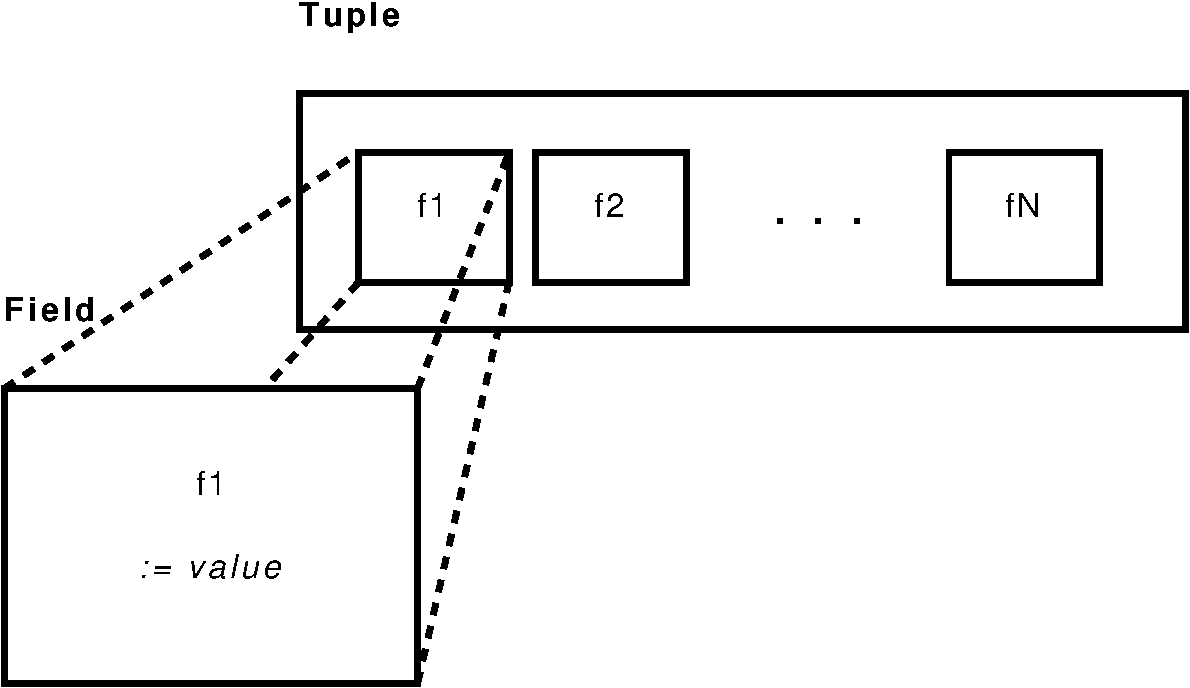
\includegraphics[width=0.7\textwidth]{diagrams/tuple_post}
  \caption[Tuple/Field structure]{The structure of a \textit{tuple} with
  \textit{fields}}
  \label{fig:method:tuple_field}
\end{center}
\end{figure}

\subsection{Semantics}
A new tuple is assumed to be created every time an old tuple needs to add or
remove one or more fields. A new field is assumed to be created for every new
value for any attribute for any tuple.

\subsection{Implications of semantics}
Any kind of projection of $x$ tuples over $n$ ``new'' attributes and $o$
``old'' attributes generates $x$ new tuples and $n$ new fields (note that
duplicates are not removed). Old fields are reused, and attribute renaming
is naturally capable of reusing old fields.

Any kind of tuple construction (e.g using the \textsf{make()} operator)
for $n$ tuples and $m$ fields generates $n$ new tuples and $n \times m$ new
fields.

\subsection{Assumptions}
TODO
\begin{itemize}
  \item Joins produserer n*m felter, for n tupler og m felter ut (iflg. T\O
  rbj\o rnsen)
  \item Diff aner vi ikke noe om
  \item Distinct aner vi ikke noe om
  \item Not inverterer
  \item Cast 
  \item Attach
\end{itemize}